(make use of HW2 and HW3) - (5 points)

\begin{enumerate}
	\item Include multiple UML diagrams to show the important parts of your system (you must have UML diagrams).
	\item Describe in a top-down manner the architecture of your system.
	\item Include enough details about the design of your system such that anyone who refers to your documentation can understand the major components of your system and how they are related.
	\item Describe how the choice of the framework influence the design of your system.
\end{enumerate}

\subsection{Class Diagram}
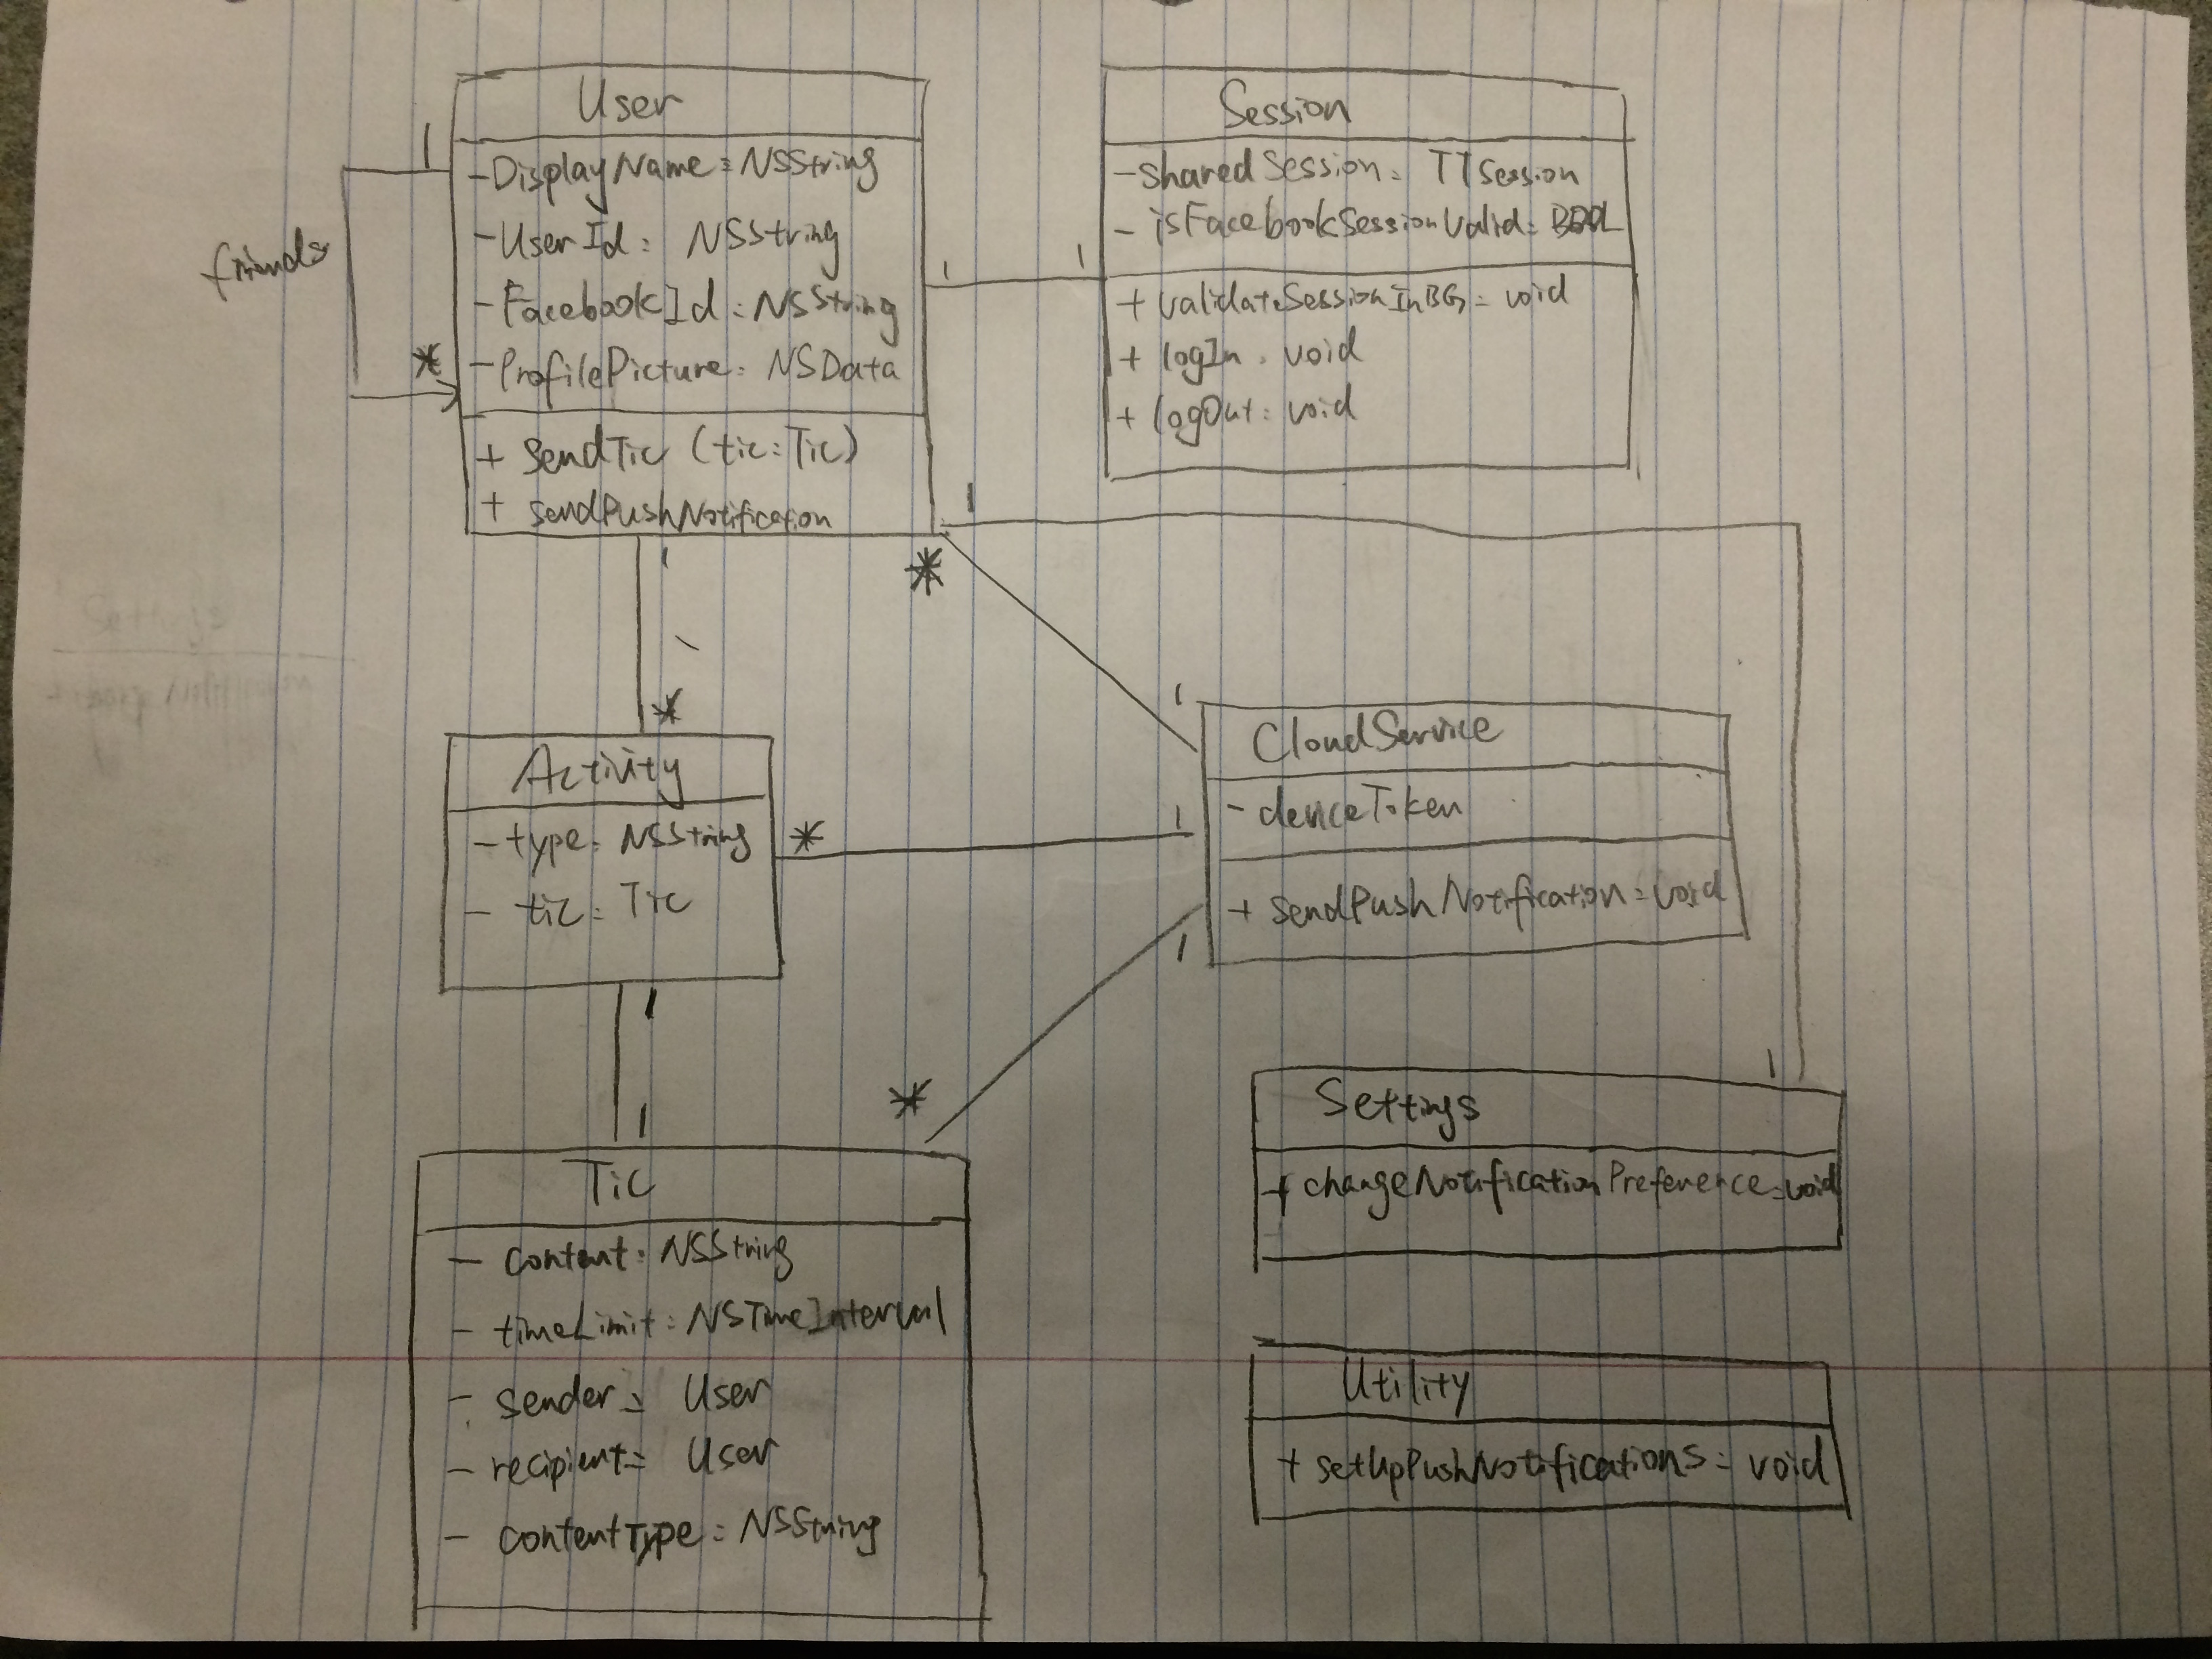
\includegraphics[width=\linewidth]{classdiagram}

\subsection{Sequence Diagrams}
\subsubsection{US1}
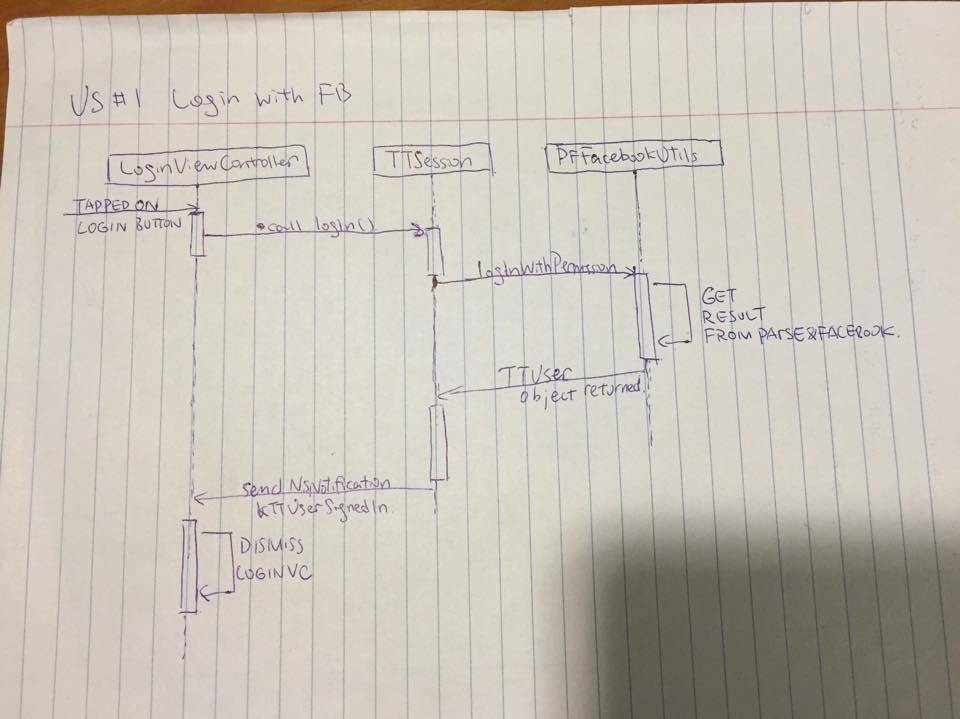
\includegraphics[width=\linewidth]{us1_sequence}

\subsubsection{US4}
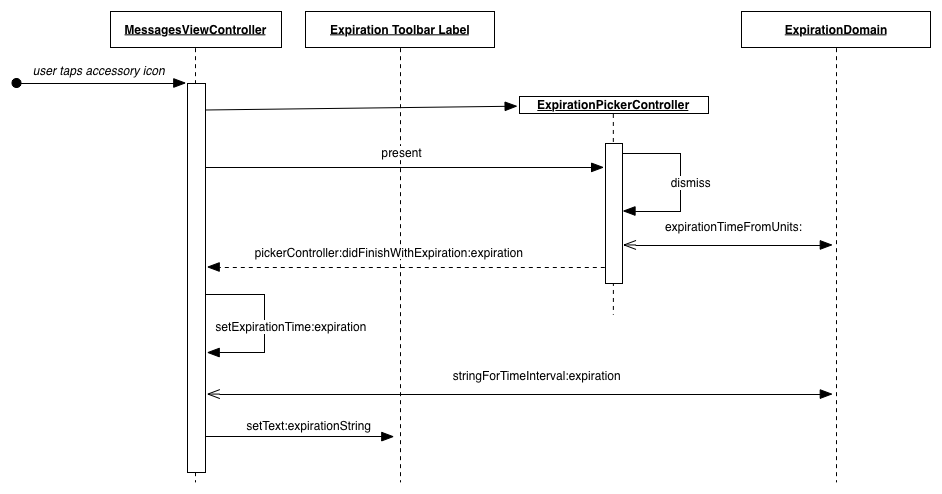
\includegraphics[width=\linewidth]{us4_sequence}

\subsubsection{US6}
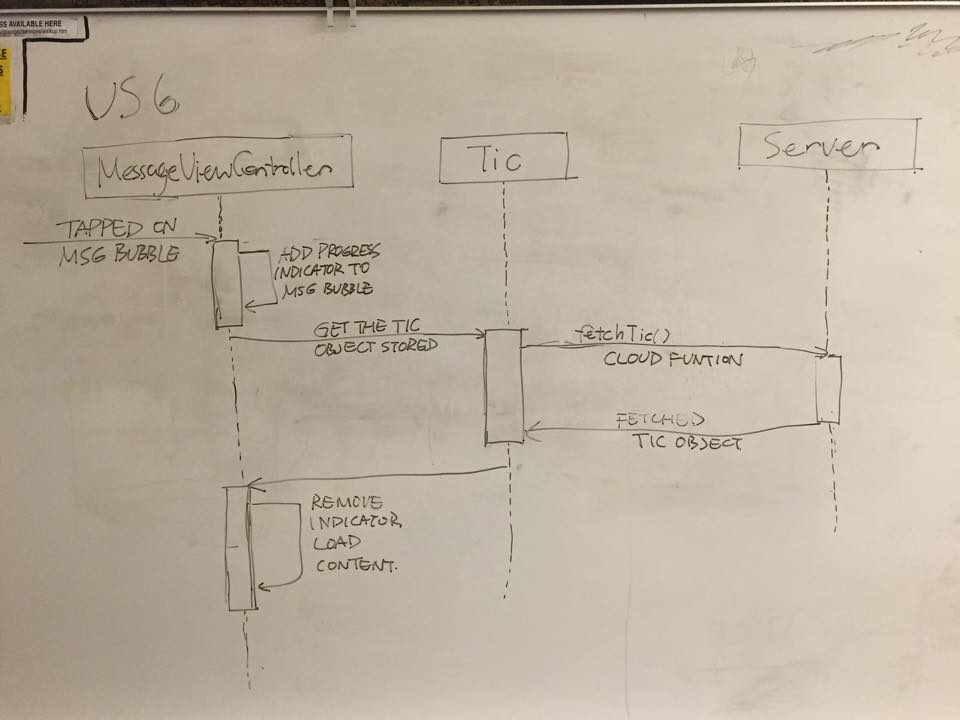
\includegraphics[width=\linewidth]{us6_sequence}

\subsubsection{US9}
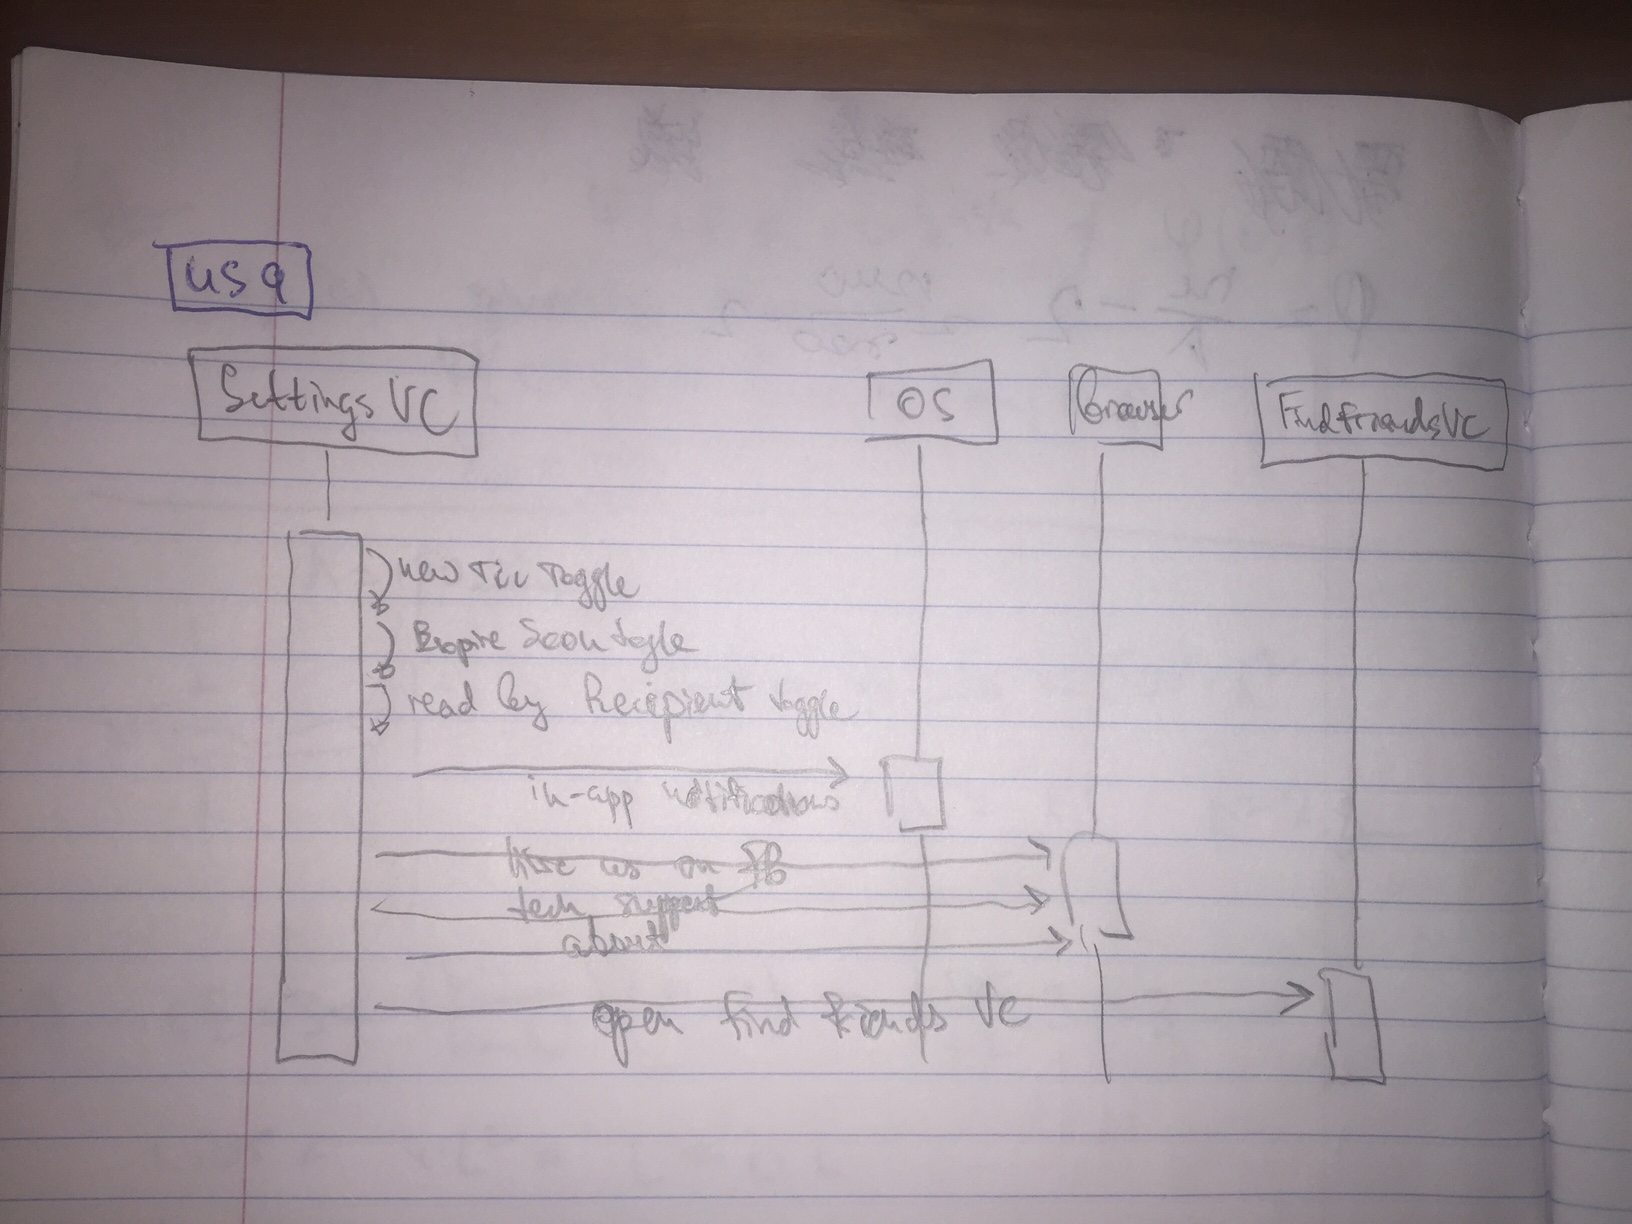
\includegraphics[width=\linewidth]{us9_sequence}

\subsubsection{US11}
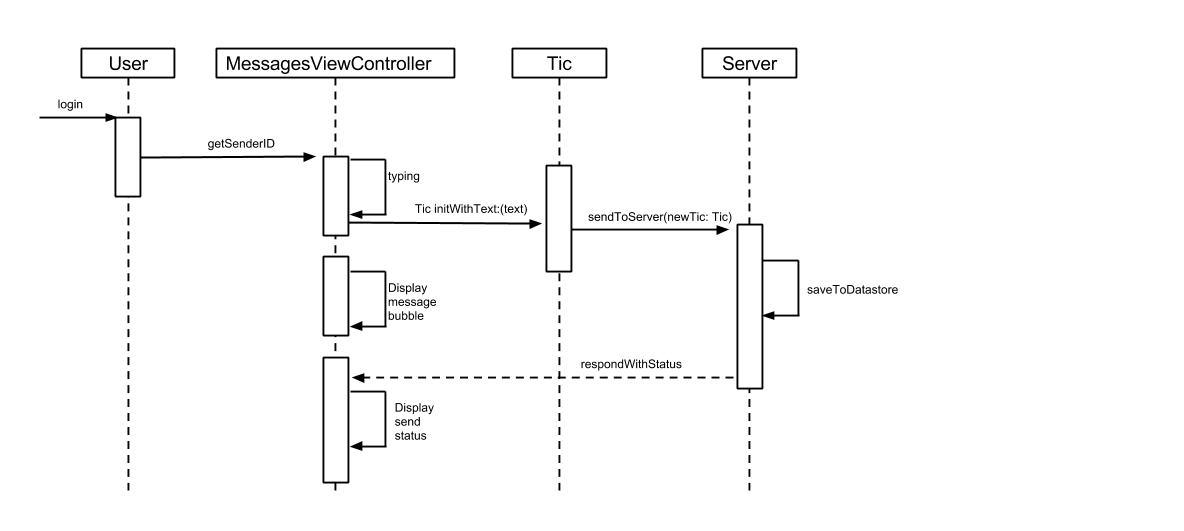
\includegraphics[width=\linewidth]{us11_sequence}

\subsubsection{US15}
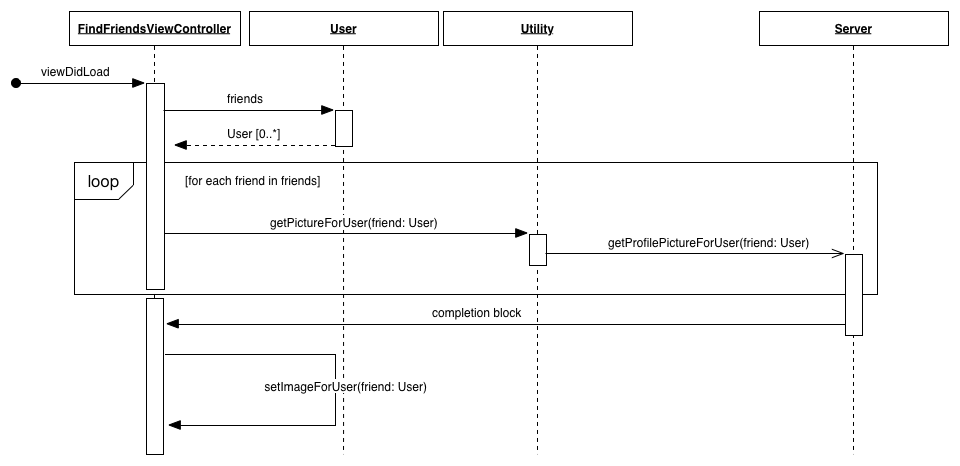
\includegraphics[width=\linewidth]{us15_sequence}
